\documentclass[11pt,a4paper]{moderncv}
\moderncvtheme[blue]{classic}

\usepackage[utf8]{inputenc}
\usepackage[inline]{enumitem}
% Marge aux 4 coins de la page, ici elles sont réduites pour gagner de la place
%\usepackage[top=1.0cm, bottom=1.0cm, left=1.6cm, right=1.6cm]{geometry}
% \usepackage[scale=0.9]{geometry}
% Largeur de la colonne de gauche pour les dates
\setlength{\hintscolumnwidth}{2.7cm}

\usepackage[T1]{fontenc}
\usepackage[french]{babel}
\usepackage{amsmath}
\usepackage{graphics}

%%%%%%%%%%%%%%%%%
\usepackage{tgtermes}
\usepackage{graphicx}
\usepackage{amssymb}
\usepackage{amstext}
\usepackage{amsmath}
\usepackage{a4wide,color}
\usepackage[final]{pdfpages} 
\usepackage{xspace}
\usepackage{anysize}
\usepackage{tabularx}
\usepackage{multirow}
\usepackage{pdfpages}
\usepackage{enumitem}
\usepackage{booktabs}
\usepackage[final]{pdfpages} 
\usepackage{microtype}
\usepackage[framemethod=tikz]{mdframed} 
\usepackage{tablefootnote} 
\makeatletter 
\AfterEndEnvironment{mdframed}{%
 \tfn@tablefootnoteprintout% 
 \gdef\tfn@fnt{0}% 
}
\makeatother 
\definecolor{color1}{rgb}{0.22,0.45,0.70}
\newcommand{\hl}[1]{\textbf{\textcolor{color1}{#1}}}
\newcommand{\hln}[1]{#1}
\renewcommand{\vec}[1]{\boldsymbol{#1}}
\newcommand*{\preduc}{\approxeq}

\newcommand*{\tool}[1]{\textsf{#1}\xspace}
\newcommand*{\caesar}{\tool{C{\ae}sar.BDD}}
\newcommand*{\its}{\tool{ITS-Tools}}
\newcommand*{\tapaal}{\tool{TAPAAL}}

\newcounter{includepdfpage}

\usepackage[
    backend=biber,
    style=alphabetic,
    natbib=true,
    sortlocale=en_US,
    url=true, 
    doi=true,
    eprint=false,
    maxnames=99
]{biblatex}
\addbibresource{candidature.bib}

\DeclareSourcemap{
  \maps[datatype=bibtex]{
    \map[overwrite]{
      \perdatasource{references.bib}
      \step[fieldset=keywords, fieldvalue={,Perhalo}, append]
    }
  }
}

\usepackage[title,titletoc]{appendix}
\renewcommand{\appendixtocname}{Annexe}
%%%%%%%%%%%%%%

\newcounter{numpart}%Création d'un compteur qui s'appelle numexos
\setcounter{numpart}{0}%initialisation du compteur
\newcommand{\partie}[1]{%Création d'une macro ayant un paramètre
\addtocounter{numpart}{1}%chaque fois que cette macro est appelée, elle ajoute 1 au compteur numexos
\textbf{\\\Large{\thenumpart.\,}\,#1 \hrulefill}%Met en rouge Exercice et la valeur du compteur appelée par \thenumeexos
}
\rfoot{Page\ \thepage}


\name{\Large Nicolas}{Amat}
\title{\normalsize  Chercheur postdoctoral\\
IMDEA Software Institute, Madrid, Espagne\\
Né le 08/02/1997 (27 ans) à Bourges (18), nationalité française\\
}   

\phone[mobile]{(+33) 6 83 32 78 84}
\email{nicolas.amat@imdea.org}
\homepage{nicolasAmat.github.io}
% \social[github]{nicolasAmat}
\extrainfo{\faGithub\href{https://github.com/nicolasAmat}{ nicolasAmat}}


\begin{document}


\thispagestyle{empty}

\begin{center}
{\small Année 2024\\---\\
\huge Candidature au poste de MCF intitulé \og Informatique - Automates, logique, données, vérification\fg\medbreak
\Large(Référence Galaxie 804)\\
\small
---\\
\Large Nicolas Amat \\
\vspace{1em}
\small Chercheur postdoctoral\\
IMDEA Software Institute, Madrid, Espagne\\
    Email : nicolas.amat@imdea.org\\
---\\
26 mars 2024}
\end{center}

\newpage

\setcounter{page}{1}
\newpage

\makecvtitle
\phantomsection\addcontentsline{toc}{chapter}{Introduction}

Actuellement en postdoctorat à l'IMDEA Software Institute de Madrid, je
travaille sur de nouvelles méthodes de résolution pour l'arithmétique de
Presburger. Mes travaux de recherche s'intéressent à la théorie et aux
applications des procédures de décision pour la vérification formelle. J'ai
effectué ma thèse de doctorat au LAAS-CNRS à Toulouse où je travaillais sur de
nouvelles méthodes pour exploiter des réductions de réseaux de Petri avec un
model-checker basé sur des méthodes SMT.\\

Je résume à la page 2 les points clés de mon dossier de candidature avant de
développer chaque partie :
\begin{itemize}
    \item formation et parcours professionnel (page~\pageref{sec:formation}),
    \item production scientifique (page~\pageref{sec:recherche}), 
    \item enseignement, ressources pédagogiques et encadrement (page~\pageref{sec:enseignements}),
    \item rayonnement scientifique et collaborations (page~\pageref{sec:rayonnement}),
    \item service académique et responsabilités (page~\pageref{sec:resp}),
    \item projet de recherche (page~\pageref{sec:projet_recherche}),
    \item projet d'enseignement (page~\pageref{sec:projet_enseignement}).\\
\end{itemize}

À la suite de ce document sont joints :
\begin{itemize}
  \item le rapport de soutenance de thèse (page~\pageref{soutenance.1}),
    \item le rapport de thèse rédigé par Mme Laure Petrucci (page~\pageref{petrucci.2}),
    \item le rapport de thèse rédigé par M. Igor Walukiewicz (page~\pageref{walukiewicz.6}),
    \item une lettre de soutien (recherche) de mes encadrants de thèse (page~\pageref{encadrants.10}),
    \item une lettre de soutien (recherche) de M. Fabrice Kordon (page~\pageref{kordon.12}),
    \item une lettre de soutien (enseignement) de M. Didier Le Botlan (page~\pageref{lebotlan.14}),
    \item une lettre de soutien (enseignement) de Mme Pauline Ribot (page~\pageref{ribot.15}).\\
\end{itemize}

\textbf{Page personnelle :} \url{https://nicolasamat.github.io/}\\

\textbf{Page GitHub :} \url{https://github.com/nicolasAmat/}
\newpage

\vspace{10pt}
\section*{Enseignement}
\vspace{10pt}

J'ai assuré un total de 146 h d'enseignements sur la période 2020--2023,
auprès d'un public varié allant de la prépa intégrée de l'INSA au master EEA de l'UPS,
en passant par le montage d'un TD spécifique sur les outils SMT au niveau M2.\\

{\small
\begin{tabular}{c @{\quad} p{13em} @{\qquad} c c c c}
\toprule
\, Niveau  & Intitulé &Formation& Nature &   \, Heures (1) \, & \, Eq. hTD (2)\,  \\
\midrule
\multicolumn{6}{l}{\textbf{2020-2021}}\\
\, L1 \,& \,Algorithmique en ADA \,&\, ing. INSA  \,&\,  TD / TP \,&\, 8,75 / 15 & 19,25\\
\midrule
\multicolumn{6}{l}{\textbf{2021-2022}}\\
\, M1 \,& \,SED, modélisation et analyse \,&\, univ. Toulouse III  \,&\,  TP \,&\, 32 & 21.33\\
\, M1 \,& \,Techniques de mises en œuvre pour les SED\,&\, univ. Toulouse III  \,&\,  TP \,&\, 30 & 20\\
\, M2 \,& \,Modèles temporels avancés \,&\, univ. Toulouse III  \,&\,  TD \,&\, 8 & 8\\
\midrule
\multicolumn{6}{l}{\textbf{2022-2023}}\\
\, L1 \,& \,Algorithmique en ADA \,&\, ing. INSA  \,&\,  TD / TP \,&\, 7,5 / 15 & 18\\
\, L3 \,& \,Expressions régulières \,&\, ing. INSA  \,&\,  TD \,&\, 5 & 5\\
\, M1 \,& \,Programmation fonctionnelle \,&\, ing. INSA  \,&\,  TP \,&\, 11 & 7,33\\
\, M2 \,& \,Modèles temporels avancés \,&\, univ. Toulouse III  \,&\,  TD \,&\, 8 & 8\\
\, M2 \,& \,SAT/SMT solving \,&\, ENAC \,&\,  TD \,&\, 6& 6\\
\bottomrule
\end{tabular}
}\\

(1) volume horaire en fonction de la nature, (2) volume horaire en équivalent TD.

\vspace{10pt}
\section*{Publications}
\vspace{10pt}

Mes travaux ont mené à 10 publications internationales : 3 articles de revue
(Fundamenta Informaticae, STTT et ToPNoC) et 7 articles de conférence parmi la
conférence de référence sur les réseaux de Petri (PETRI NETS), celle de
référence en model-checking (SPIN) et des conférences plus généralistes de rang
A tel que TACAS et FM.

\vspace{10pt}
\section*{Logiciels}
\vspace{10pt}

J'ai développé 4 outils open source. Un de ces outils est
\textsf{SMPT}, un model-checker de réseaux de Petri qui s'est distingué au Model
Checking Contest (compétition internationale d'outils de model checking) en
obtenant la médaille de bronze en 2022 et 2023 dans la catégorie
``accessibilité''.



\label{sec:cv}
\vspace{-1cm}

\newpage
\partie{Formation et parcours professionnel}
\phantomsection\addcontentsline{toc}{chapter}{Formation et parcours professionnel}

\section{Parcours}
\label{sec:formation}
\vspace{5pt}

\cventry{2023 - 2024\hfill}{Postdoctorat}{}{}{}{}
\cvitem{Sujet}{\emph{Méthodes de résolution pour l'arithmétique de Presburger}}
\cvitem{Laboratoire}{IMDEA Software Institute, Madrid, Espagne}
\cvitem{Démarage}{Novembre 2023}
\cvitem{Encadrants}{M. Pierre Ganty (Associate Research Professor, IMDEA Software Institute)}
\cvitem{}{M. Alessio Mansutti (Associate Research Professor, IMDEA Software Institute)}
\vspace{10pt}


\cventry{2020 - 2023 \hfill}{Doctorat}{Bourse ministérielle}{}{}{}
\cvitem{Titre}{\emph{\mbox{A Polyhedral Framework for Reachability Problems in Petri Nets}}}
\cvitem{Spécialité}{Informatique et Télécommunications}
\cvitem{Laboratoire}{Laboratoire d'Analyse et d'Architecture des Systèmes (LAAS-CNRS)}
\cvitem{Établissement}{Institut National des Sciences Appliquées de Toulouse (INSA Toulouse)}
\cvitem{Période}{1\ier octobre 2020 -- 31 octobre 2023}
\cvitem{Soutenance}{4 décembre 2023}
\cvitem{Directeurs}{M. François Vernadat (PU, INSA Toulouse)}
\cvitem{}{M. Didier Le Botlan (MCF, INSA Toulouse)}
\cvitem{}{M. Silvano Dal Zilio (CR, CNRS)}
\cvitem{Rapporteurs}{Mme Laure Petrucci (PU, Univ. Sorbonne Paris Nord)}
\cvitem{}{M. Igor Walukiewicz (DR, CNRS)}
\cvitem{Examinateurs}{Mme Béatrice Bérard (Prof. émerite, Sorbonne Université)}
\cvitem{}{M. Fabrice Kordon (PU, Sorbonne Université)}
\cvitem{Président}{M. Loïc Hélouët (DR, INRIA)}
\cvitem{Manuscrit}{\url{https://theses.hal.science/tel-04458457}}
\cvitem{Transparents}{\url{https://nicolasamat.github.io/Slides_PhD.pdf}}
\vspace{10pt}

\cventry{2019 - 2020 \hfill}{Master of Science in Informatics at Grenoble (MoSIG)}{}{}{}{}
\cvitem{Université}{Université Grenoble Alpes}
\cvitem{Spécialité}{High-confidence Embedded and Cyberphysical Systems (HECS)}
\cvitem{Mention}{Très bien (major de promotion)}
\cvitem{Mémoire}{\emph{A new approach for the symbolic model checking of Petri nets}}
\cvitem{Soutenance}{23 juin 2020}
\cvitem{Directeurs}{M. Silvano Dal Zilio (CR, CNRS)}
\cvitem{}{M. Hubert Garavel (DR, INRIA)}
\cvitem{Rapporteur}{M. Yann Thierry-Mieg (MCF, Sorbonne Université)}
\cvitem{Examinateurs}{M. Akram Idani (MCF, Grenoble INP -- ENSIMAG)}
\cvitem{}{Mme Laurence Pierre (PU, Université Grenoble Alpes)}
\cvitem{Financement}{Bourse d'excellence du LabEx PERSYVAL-Lab}
\newpage

\cventry{2017 - 2020 \hfill}{Ingénieur en Informatique}{Grenoble INP -- ENSIMAG}{}{}{}
\cvitem{Spécialité}{Ingénierie des Systèmes d'Information (ISI)}
\cvitem{Mention}{Très bien (major de promotion)}
\vspace{10pt}

\cventry{2015 - 2017 \hfill}{Classes Préparatoires}{La Prépa des INP de Toulouse}{}{}{}


\section{Expériences professionnelles}

\cventry{2019 \hfill}{Stage assistant ingénieur}{ARM Ltd.}{Cambridge (UK)}{}{}
\cvitem{Contribution}{J'ai réalisé un ensemble de modifications du pilote des
GPU Mali d'Arm pour permettre son exécution sur User-Mode Linux (UML), un noyau
Linux compilé qui peut être exécuté dans l'espace utilisateur comme un simple
programme. J'ai également proposé un correctif du noyau Linux pour fournir sur
UML un accès direct à la mémoire (DMA) et une compatibilité avec devicetree
(structure de donnée décrivant les composants matériels).}
\cvitem{Encadrant}{M. Chris Diamand (Senior Software Engineer, ARM Ltd.)}
\cvitem{Durée}{3 mois}
\vspace{10pt}

\cventry{2019 \hfill}{Introduction à la recherche en laboratoire}{LIG}{Grenoble (France)}{}{}
\cvitem{Contribution}{J'ai réalisé une formalisation de la logique de séparation
à l'aide de l'assistant de preuve Isabelle/HOL ainsi que la preuve de résultats
de réécriture de formules issus d'un article intitulé \og The
Bernays-Schönfinkel-Ramsey Class of Separation Logic on Arbitrary Domains \fg.}
\cvitem{Encadrants}{M. Mnacho Echenim (PU, Grenoble INP -- ENSIMAG)}
\cvitem{}{M. Nicolas Peltier (CR, CNRS)}
\cvitem{Durée}{Une journée par semaine durant un semestre}
\vspace{10pt}

\cventry{2017 \hfill}{Stage en laboratoire}{IRIT}{Toulouse (France)}{}{}
\cvitem{Contribution}{J'ai réalisé des améliorations de sécurité dans XPIR, un
logiciel open source permettant à un utilisateur de télécharger de manière
secrète un élément d'une base de données (le serveur de la base de données sait
qu'il a envoyé un élément à l'utilisateur, mais ne sait pas lequel). Un tel
protocole est appelé Private Information Retrieval (PIR) et dans le cas de XPIR
ce dernier repose sur un chiffrement homomorphe.}
\cvitem{Encadrant}{M. Carlos Aguilar Melchor (MCF, Toulouse INP -- ENSEEIHT)}
\cvitem{Durée}{2 mois}


\section{Compétences techniques}

\cvitem{Programmation}{OCaml, Python, C, Java, Ada}
\cvitem{Solveurs}{z3, MiniZinc}
\cvitem{Model-checking}{Uppaal, LNT, Tina (Selt \& Muse)}
\cvitem{Asst. de preuve}{Isabelle/HOL}
\cvitem{Script}{Shell}
\cvitem{Hardware}{VHDL}




\newpage
\partie{Production scientifique}
\label{sec:recherche}


\vspace{10pt}
\section*{Description synthétique de mes travaux passés}
\vspace{10pt}

Mes travaux de recherche s'intéressent à la théorie et aux applications des
procédures de décision pour la vérification formelle. J'ai effectué ma thèse de
doctorat au LAAS-CNRS à Toulouse où je travaillais sur de nouvelles méthodes
pour exploiter des réductions de réseaux de Petri avec un model-checker basé sur
des méthodes SMT. Je travaille actuellement sur l'arithmétique de Presburger
dans le cadre d'un postdoctorat effectué à l'IMDEA Software Institute de Madrid

\vspace{10pt}
\subsection*{Thèse de doctorat}
\vspace{10pt}


Au cours de ma thèse de doctorat, j'ai proposé et étudié une méthode pour
contrôler l'explosion combinatoire lors de la vérification de problèmes
d'accessibilité sur les réseaux de Petri basée sur des réductions structurelles
appelées réductions polyédriques~\cite{amat_combination_2021,amat_polyhedral_2022}. L'approche est basée
sur une abstraction de l'espace d'états qui combine réductions structurelles et
contraintes arithmétiques sur le marquage des places.\\

La correction de cette méthode est basée sur une nouvelle notion d'équivalence
comportementale entre les réseaux. Combiné avec un model-checker basé sur des
méthodes SMT, je propose de transformer un problème d'accessibilité sur un
réseau de Petri en la vérification d'une propriété d'accessibilité sur une
version réduite de ce réseau~\cite{amat_combination_2021,amat_polyhedral_2022}. En exploitant un lien
avec une classe de réseaux de Petri qui ont un ensemble d'accessibilité
définissable par l'arithmétique de Presburger, j'ai également proposé
une procédure automatisée pour prouver qu'une telle abstraction est
correcte~\cite{amat_automated_2023}.\\

De plus, j'ai développé une structure de données, appelée Token Flow Graph
(TFG), qui capture la structure particulière des contraintes résultant des
réductions polyédriques~\cite{amat_accelerating_2021,amat_leveraging_2022}. J'ai exploité les TFGs
pour résoudre efficacement deux problèmes. Premièrement, pour éliminer les
quantificateurs, qui apparaissent lors de notre transformation, dans la formule
à vérifier sur le réseau réduit~\cite{amat_project_2024}. Deuxièmement, pour le
calcul de la relation de concurrence d'un réseau, c'est-à-dire énumérer toutes
les paires de places qui peuvent être marquées simultanément dans un marquage
accessible. Ce travail a conduit à une collaboration avec l'équipe CONVECS de
INRIA Grenoble~\cite{amat_toolchain_2023}.\\

J'ai appliqué mon approche à plusieurs procédures de model-checking symboliques.
Un des résultats de ce travail est la définition d'une nouvelle procédure de
semi-décision pour la vérification de propriétés d'accessibilité sur les réseaux
de Petri, basée sur la méthode Property Directed Reachability
(PDR)~\cite{amat_property_2022}. Une particularité de cette méthode PDR réside
dans sa capacité à générer des certificats de verdict en arithmétique de
Presburger qui peuvent être vérifiés à l'aide d'un solveur SMT externe.\\

Je valorise une approche de la recherche qui combine des avancées théoriques avec
des implémentations concrètes. J'ai mis en œuvre mes résultats et mes algorithmes
dans quatre outils open source : \textsf{SMPT} pour vérifier des propriétés
d'accessibilité~\cite{amat_smpt_2023} ; \textsf{Kong} pour accélérer le calcul de places concurrentes~\cite{amat_kong_2022}
; \textsf{Octant} pour l'élimination de quantificateurs ; et \textsf{Reductron} pour
prouver automatiquement la correction de réductions polyédriques. J'ai étudié
leur efficacité dans le cadre d'évaluations expérimentales approfondies, à la
fois pour des réseaux bornés et non bornés, en utilisant les modèles et formules
fournies par le Model Checking Contest
(MCC)\footnote{\url{https://mcc.lip6.fr}}, une compétition annuelle et
internationale pour les outils de model-checking. Cela m'a conduit à participer
à la catégorie ``accessibilité'' des trois dernières éditions du MCC. Mon outil,
\textsf{SMPT}, a obtenu la médaille de bronze lors des deux dernières éditions
(2022 et 2023).

\vspace{10pt}
\subsection*{Postdoctorat}
\vspace{10pt}

Dans le cadre de mon postdoctorat réalisé à l'IMDEA Software Institute de
Madrid, je m'intéresse à la résolution de fragments spécifiques de
l'arithmétique de Presburger. D'un point de vue théorique, l'arithmétique de
Presburger est connue pour être décidable. Cependant, tout comme pour le
problème d'accessibilité sa complexité théorique (quelque part entre 2EXPTIME et
3EXPTIME) fait de sa résolution un véritable défi. Une conséquence pratique de
cette \og complexité inhérente \fg est qu'une stratégie intéressante consiste à
essayer d'améliorer les performances sur certains fragments particuliers pour
traiter de grandes formules provenant de problèmes de vérification concrets.\\

Si nous nous limitons au fragment sans quantificateur (également connu sous le
nom de Quantifier-Free Linear Integer Arithmetic, ou QF-LIA en abrégé), les
progrès récents des solveurs SMT permettent désormais de développer des
techniques de vérification efficaces pour le model-checking, l'interprétation
abstraite, etc. Cependant, ce fragment n'est pas assez expressif pour de
nombreux problèmes concrets, tels que le raisonnement sur différentes bases, la
recherche de points fixes, ou la vérification d'interpolants, qui nécessitent
souvent l'ajout de quantificateurs existentiels et peuvent être exprimés comme un
problème d'inclusion entre formules.\\

Dans ce contexte, je développe de nouvelles méthodes de vérification pour
des fragments spécifiques. Un premier fragment intéressant, comme mentionné
précédemment, est l'inclusion de formules existentielles. Fondamentalement,
une formule existentielle implique-t-elle (ou est-elle équivalente à) une autre
? Plus abstraitement, ce fragment peut être considéré comme un problème
d'inclusion de langage.  J'ai récemment développé une approche qui repose sur
un cadre théorique pour l'inclusion de deux langages, basé sur la notion de
quasi-ordre, qui réduit le problème à un nombre fini de questions
d'appartenance. 
% Nos premiers résultats montrent que cette
% approche innovante est plus efficace dans la pratique que les approches
% \og géométriques\fg  plus générales.\\

\vspace{10pt}
\subsection*{Autres travaux}
\vspace{10pt}

Durant mes études à l'ENSIMAG, j'ai travaillé avec de deux mes enseignants sur
la formalisation de la logique de séparation dans l'assistant de preuve
Isabelle/HOL, et la preuve de résultats de réécriture de formules. Ce travail
est disponible
librement~\footnote{\url{https://github.com/nicolasAmat/Separation-Logic-Formalization}}.

\vspace{10pt}
\section*{Liste des publications}
\label{sec:publications}
\vspace{10pt}

Mes travaux ont mené à 10 publications internationales (dont je suis le
co-auteur principal) : 3 articles de revue (Fundamenta Informaticae, STTT et
ToPNoC) et 7 articles de conférence parmi des conférences généralistes de rang A
tel que TACAS et FM (taux d'acceptation inférieurs à 30\%), la conférence VMCAI,
la conférence de référence sur les réseaux de Petri (PETRI NETS) et celle de
référence en model-checking (SPIN). À noter que deux autres articles de revue
sont en cours de publication (un accepté et un autre soumis).
\medbreak

Ci-après une liste de mes publications classées par type de communication et
par ordre chronologique. Le symbole ($\bigstar$) indique que j'ai choisi la
publication comme publication de référence (5 au total).
% Le symbole ($\bigstar$) indique que j'ai choisi la
% publication comme publication de référence (5 au total).

\vspace{10pt}
\subsection*{Revues internationales avec comité de lecture}
\vspace{10pt}

\begin{enumerate}
  \item ($\bigstar$) \cite{amat_polyhedral_2022} \fullcite{amat_polyhedral_2022} 
  \begin{mdframed}
    Cet article de revue introduit le cade théorique des réductions polyédriques
    appliquées à la vérification de propriétés d'accessibilité. J'y propose une
    nouvelle notion d'équivalence comportementale entre les réseaux, nommée
    \emph{équivalence polyédrique}, et je montre comment la combiner avec un
    model-checker basé sur des méthodes SMT. Ce travail a lancé le développement
    de mon outil \textsf{SMPT}, dans lequel j'ai appliqué mon approche à
    plusieurs procédures de model-checking symbolique. Les résultats
    expérimentaux ont montré que l'approche fonctionne bien sur le jeu de
    données du Model Checking Contest (reconnu par ma communauté), même
    lorsqu'une quantité modérée de réductions s'applique.
  \end{mdframed}
  \smallbreak
  % \textcolor{gray}{\textbf{Contribution :} Dans cet article de journal j'ai
  % défini une nouvelle méthode pour tirer parti des réductions de réseaux en
  % combinaison avec un model checker basé sur des méthodes SMT. L'approche
  % consiste à transformer un problème d'accessibilité sur un réseau de Petri en
  % la vérification d'une propriété d'accessibilité sur une version réduite de ce
  % réseau. Cette méthode repose sur une nouvelle abstraction de l'espace d'états
  % basée sur des systèmes de contraintes, appelée reduction polyédrique. Nous
  % prouvons la correction de cette méthode en utilisant une nouvelle notion
  % d'équivalence entre les réseaux. Notre approche a été mise en œuvre dans un
  % outil, appelé \textsf{SMPT}, qui fournit deux procédures principales : Bounded
  % Model Checking (BMC) et Property Directed Reachability (PDR). Nous avons testé
  % \textsf{SMPT} sur une large collection de problèmes utilisés au Model Checking
  % Contest. Nos résultats expérimentaux montrent que notre approche fonctionne
  % bien, même lorsque nous n'avons qu'une quantité modérée de réductions.}
	
  \item \cite{amat_leveraging_2022} \fullcite{amat_leveraging_2022} 
  % \smallbreak
  
  % \textcolor{gray}{\textbf{Contributions :} Dans cet article de revue je
	% propose une nouvelle structure de données, appelée Token Flow Graph (TFG), qui
	% capture la structure particulière des contraintes apparaissant dans les
	% réductions polyédriques. Nous utilisons les TFGs pour résoudre efficacement
	% deux problèmes d'accessibilité : d'abord pour vérifier l'accessibilité d'un
	% marquage donné et ensuite pour calculer la relation de concurrence d'un
	% réseau, c'est-à-dire énumérer toutes les paires de places qui peuvent être
	% marqués simultanément dans un marquage accessible. Nos algorithmes sont
	% implantés dans un outil, appelé \textsf{Kong}, que nous évaluons sur une
	% large collection de modèles utilisés lors du Model Checking Contest. Nos
	% expérimentations montrent que l'approche fonctionne bien, même lorsqu'une quantité
	% modérée de réductions s'applique.}
  \smallbreak
	\item ($\bigstar$) \cite{amat_toolchain_2023} \fullcite{amat_toolchain_2023}
  \begin{mdframed}
    Cet article publié dans la revue ToPNoC (Transactions on Petri Nets and Other
  Models of Concurrency) est le fruit de ma collaboration avec l’équipe CONVECS de
  INRIA Grenoble, sur le problème des places concurrentes. On y présente notre
  approche, combinant l'outil \caesar, qui fait partie de la boîte à outils
  \textsf{CADP}, avec les Token
  Flow Graphs qui sont une structure de données capturant la structure
  particulière des contraintes résultant de réductions polyédriques. Cette
  collaboration m’a également amené à développer l’outil
  \textsf{Kong}.
  \end{mdframed}
\end{enumerate}


\vspace{10pt}
\subsection*{Conférences internationales avec comité de lecture}
\vspace{10pt}
\begin{enumerate}
  \setcounter{enumi}{3}
  \item  \cite{amat_combination_2021} \fullcite{amat_combination_2021}
  \smallbreak
  \emph{Article sélectionné parmi les meilleures contributions pour être étendu en journal.}
  \smallbreak
  \item \cite{amat_accelerating_2021} \fullcite{amat_accelerating_2021}
  \smallbreak
  \emph{Article sélectionné parmi les meilleurs contributions pour être étendu en journal.}
  \smallbreak
  \item ($\bigstar$) \cite{amat_property_2022} \fullcite{amat_property_2022}
  \begin{mdframed}
    Dans cet article j'ai proposé un nouvel algorithme, qui est une procédure de
  semi-décision pour le problème d'accessibilité basée sur la méthode Property
  Directed Reachability (PDR), parfois aussi appelée IC3. Une caractéristique
  distinctive de cette extension de PDR aux réseaux de Petri est sa capacité à
  générer un \emph{certificat d'invariance}, sous la forme d'un invariant
  inductif de Presburger, lorsque nous constatons qu'une propriété est vérifiée
  par tous les états accessibles. J'ai choisi de présenter cette contribution
  car, à ma connaissance, elle est la seule méthode à fournir de tels
  certificats de manière effective dans le cas général (bien que l'existence
  théorique de tels certificats fût prouvée par Leroux en 2010).
  \end{mdframed}
  \smallbreak
  % \textcolor{gray}{\textbf{Contributions :} Dans cet article je propose une
  % procédure de semi-décision pour vérifier des propriétés d'accessibilité dans
  % les réseaux de Petri, basée sur la méthode PDR (Property Directed
  % Reachability). Nous définissons trois versions différentes, qui sont capables
  % de traiter des problèmes d'une difficulté croissante. J'ai implanté ces
  % méthodes dans mon model checker SMPT et nous donnons des preuves empiriques
  % que notre approche peut traiter problèmes difficiles ou impossibles à vérifier
  % avec les outils de l'état de l'art.}
  % \smallbreak
  \item \cite{amat_kong_2022} \fullcite{amat_kong_2022}
  \smallbreak
  \emph{Article sélectionné parmi les meilleurs contributions pour être étendu en journal.}
  \smallbreak
  \item ($\bigstar$) \cite{amat_smpt_2023} \fullcite{amat_smpt_2023}
  \begin{mdframed}
    Dans cet article je présente mon outil \textsf{SMPT} (\emph{Satisfiability
    Modulo Petri Nets}), sous licence libre (GPLv3). \textsf{SMPT} est un
    model-checker pour la vérification de propriétés d'accessibilité dans les
    réseaux de Petri, basé sur des méthodes SMT. Il a la particularité de tirer
    parti des réductions polyédriques. Cet outil a une importance particulière car
    il est le fondement de mes travaux expérimentaux de thèse et représente plus de
    $4\,500$ lignes de code (et $5\, 000$ lignes de commentaires et documentation). 
  \end{mdframed}
  \smallbreak
  \item \cite{amat_automated_2023} \fullcite{amat_automated_2023}
  \smallbreak
  \emph{Article sélectionné parmi les meilleurs contributions pour être étendu en journal.}
  \smallbreak
  % \textcolor{gray}{\textbf{Contributions :} Dans cet article je propose une
  % procédure automatisée pour prouver la corrections d'équivalences
  % polyédriques pour les réseaux de Petri. Mon approche repose sur un encodage
  % en un ensemble de formules SMT dont la satisfaction implique que l'équivalence
  % est correcte. La difficulté, dans ce contexte, provient du fait que nous devons
  % traiter des systèmes à états infinis. Pour la complétude, nous exploitons un
  % lien avec une classe de réseaux de Petri qui ont un ensemble d'accessibilité
  % définissables par l'arithmétique de Presburger. J'ai implanté
  % cette procédure dans un outil appelé \textsf{Reductron}.}
  % \smallbreak
  \item ($\bigstar$) \cite{amat_project_2024} \fullcite{amat_project_2024}
  \begin{mdframed}
    Cet article est représentatif de mon projet de recherche, mêlant vérification
  formelle et raisonnement automatisé. J'y ai proposé une méthode pour vérifier
  des propriétés d'accessibilité dans les réseaux de Petri en tirant parti de
  réduction polyédrique de manière transparente, comme une étape de prétraitement
  pour n'importe quel outil de model-checking. Mon approche est basée sur une
  nouvelle procédure qui peut projeter une propriété, d'un réseau de Petri
  initial, en une formule équivalente qui ne fait référence qu'à sa version
  réduite. Cette projection est définie comme une procédure d'élimination de
  quantificateurs pour l'arithmétique de Presburger, adaptée au fragment
  spécifique résultant de réductions. Les résultats expérimentaux ont montré
  que (1) sur notre fragment, mon outil de projection \textsf{Octant} est
  plus efficace que les outils généraux pour l'arithmétique de Presburger ; et (2)
  les réductions polyédriques sont efficaces sur un grand nombre de propriétés
  d'accessibilité, orthogonales aux optimisations existantes et que leurs
  avantages se combinent avec d'autres optimisations et model-checkers.
  \end{mdframed}
\end{enumerate}

\vspace{10pt}
% \vspace{1em}
\subsection*{Preprints}
\vspace{5pt}
\begin{enumerate}
  \setcounter{enumi}{10}
  \item \fullcite{preprint_1}\smallbreak
  \item \fullcite{preprint_2}
\end{enumerate}



\vspace{5pt}
\subsection*{Poster}
\vspace{5pt}
\begin{enumerate}
  \setcounter{enumi}{12}
  \item \fullcite{poster}
\end{enumerate}
\vspace{5pt}


\section*{Logiciels}
\vspace{10pt}
J'assure le développement et la maintenance de 4 outils open source (licence
GPLv3), en liens directs avec mes travaux de thèse, que je décris ci-dessous.
Pour chaque logiciel, la page GitHub correspondante contient le manuel
d'utilisation.
\vspace{10pt}

\begin{enumerate}
  \setcounter{enumi}{13}
  \item \textbf{SMPT: The Satisfiability Modulo Petri Nets Model Checker.}\\
  \url{https://github.com/nicolasAmat/SMPT}
  \begin{mdframed}
  Un model-checker basé sur des méthodes SMT pour les réseaux de Petri, axé sur
  les problèmes d'accessibilité, qui tire parti de réductions polyédriques.
  \textsf{SMPT} a participé aux trois dernières éditions du Model Checking
  Contest dans la catégorie \og accessibilité \fg et a obtenu la médaille de bronze
  en 2022 et 2023.
  \smallbreak
  \emph{Environ $4\ 500$ lignes de code et $5\, 000$ lignes de commentaire.}
  \end{mdframed}

  \item \textbf{Octant: The Reachability Formula Projector.}\\
  \url{https://github.com/nicolasAmat/Octant}
    \begin{mdframed}
  Un outil pour projeter des propriétés d'accessibilité d'un réseaux de Petri
  sur sa version réduite. Cet outil est utilisé dans le fonctionnement interne
  du model-checker \textsf{SMPT}.
  \smallbreak
  \emph{Environ $1\,500$ lignes de code.}
    \end{mdframed}
  
  \item \textbf{Kong: The Koncurrent Places Grinder.}\\
  \url{https://github.com/nicolasAmat/Kong}
  \begin{mdframed}
  Un outil pour accélérer le calcul de la relation de concurrence d'un réseau de
  Petri en utilisant des réductions polyédriques. Cet outil a été réalisé dans
  le cadre d'une collaboration avec l'équipe CONVECS de INRIA Grenoble.
  \smallbreak
  \emph{Environ $1\ 000$ lignes de code.}
  \end{mdframed}
  \newpage

  \item \textbf{Reductron: The Polyhedral Abstraction Prover.}\\
  \url{https://github.com/nicolasAmat/Reductron}
  \begin{mdframed}
  Un outil pour prouver automatiquement la correction d'équivalences
  polyédriques pour les réseaux de Petri.
  \smallbreak
  \emph{Environ $1\ 000$ lignes de code.}
  \end{mdframed}
\end{enumerate}
\vspace{10pt}



\section*{Science ouverte}
\vspace{10pt}
J'accorde une grande importance aux aspects \og science ouverte \fg dans mes travaux
de recherche. Cela s'est traduit par la développement de quatre outils open
source (décrits précédemment), la production de jeux de données, la mise à
disposition d'artefacts pour faciliter la reproduction de mes résultats et la
participation aux trois dernières éditions du Model Checking Contest, une
compétition internationale d'outils de model-checking pour la vérification de
systèmes concurrents. Ci-dessous je liste ces contributions.

\vspace{10pt}
\subsection*{Jeux de données}
\vspace{10pt}
J'ai contribué à la proposition de plusieurs modèles utilisés dans le benchmark du Model Checking Contest, en 
définissant trois modèles. J'ai également soumis une base de donnée de formules ajoutées au répertoire SMT-LIB
utilisé durant la compétition SMT-COMP.
\vspace{5pt}
\begin{enumerate}
  \setcounter{enumi}{17}
  \item \fullcite{amat_cryptominer_2023}\smallbreak
  \item \fullcite{amat_pgcd_2023}\smallbreak
  \item \fullcite{amat_murphy_2023}\smallbreak
  \item \fullcite{amat_qf-lia_2023}
\end{enumerate}

\vspace{10pt}
\subsection*{Artefacts}
\vspace{5pt}

J'ai fourni trois artefacts sur la plateforme \textsf{Zenodo}, pour les
conférences ayant une évaluation d'artefacts dans leur processus de soumission
(TACAS, FM et VMCAI). J'ai également produit un artefact couvrant l'ensemble de
mes travaux de thèse. L'objectif de ces artefacts est de permettre à la
communauté de reproduire mes résultats expérimentaux ainsi que de fournir un
environnement fonctionnel pour mes outils.
\vspace{1pt}
\begin{enumerate}
  \setcounter{enumi}{21}
  \item \fullcite{zenodo_artifact_2022}\smallbreak
  \item \fullcite{zenodo_artifact_2023}\smallbreak
  \item \fullcite{zenodo_artifact_2024}\smallbreak
  \item \fullcite{zenodo_artifact}
\end{enumerate}
\newpage


\subsection*{Compétition}
\vspace{10pt}

Ci-dessous je liste les références à mes trois participations au Model Checking Contest.
\vspace{10pt}
\begin{enumerate}
  \setcounter{enumi}{25}
  \item \textbf{2021.} \fullcite{kordon_complete_2021}\smallbreak
  \item \textbf{2022.} \fullcite{kordon_complete_2022}\smallbreak
  \item \textbf{2023.} \fullcite{kordon_complete_2023}
\end{enumerate}



\newpage
\partie{Enseignement, ressources pédagogiques et encadrement}
\label{sec:enseignements}


\vspace{10pt}
\section*{Enseignement}\label{sec:tab}
\vspace{10pt}

Dans cette section je décris les enseignements que j'ai effectués durant mes trois
années de thèse en tant que vacataire. Ces enseignements sont de tous niveaux
(L1 à M2) et ont été réalisés dans trois établissements différents (INSA
Toulouse, Université Toulouse III et ENAC).\\

{\small
\begin{tabular}{c @{\quad} p{13em} @{\qquad} c c c c}
\toprule
\, Niveau  & Intitulé &Formation& Nature &   \, Heures (1) \, & \, Eq. hTD (2)\,  \\
\midrule
\multicolumn{6}{l}{\textbf{2020-2021}}\\
\, L1 \,& \,Algorithmique en ADA \,&\, ing. INSA  \,&\,  TD / TP \,&\, 8,75 / 15 & 19,25\\
\midrule
\multicolumn{6}{l}{\textbf{2021-2022}}\\
\, M1 \,& \,SED, modélisation et analyse \,&\, univ. Toulouse III  \,&\,  TP \,&\, 32 & 21.33\\
\, M1 \,& \,Techniques de mises en œuvre pour les SED\,&\, univ. Toulouse III  \,&\,  TP \,&\, 30 & 20\\
\, M2 \,& \,Modèles temporels avancés \,&\, univ. Toulouse III  \,&\,  TD \,&\, 8 & 8\\
\midrule
\multicolumn{6}{l}{\textbf{2022-2023}}\\
\, L1 \,& \,Algorithmique en ADA \,&\, ing. INSA  \,&\,  TD / TP \,&\, 7,5 / 15 & 18\\
\, L3 \,& \,Expressions régulières \,&\, ing. INSA  \,&\,  TD \,&\, 5 & 5\\
\, M1 \,& \,Programmation fonctionnelle \,&\, ing. INSA  \,&\,  TP \,&\, 11 & 7,33\\
\, M2 \,& \,Modèles temporels avancés \,&\, univ. Toulouse III  \,&\,  TD \,&\, 8 & 8\\
\, M2 \,& \,SAT/SMT solving \,&\, ENAC \,&\,  TD \,&\, 6& 6\\
\bottomrule
\end{tabular}
}
\medbreak

(1) volume horaire en fonction de la nature, (2) volume horaire en équivalent TD.

\vspace{10pt}

\underline{\textbf{Total d'heures effectuées :}} 146,25 h (112,91 h équivalent TD).\\

Ci-dessous une description détaillée de mes enseignements par établissement.\\

\subsection*{Institut National de Sciences Appliquées de Toulouse (INSA)}

\vspace{10pt}
\textbf{Algorithmique en ADA}.\medbreak 

Niveau : L1 -- 2020/2021 : 8,75 hTD et 15 hTP -- 2022/2023 : 7,5 hTD et 15 hTP.
% \medbreak 
\begin{mdframed}
  L'objectif de ce cours est d'enseigner les bases de l'algorithmique en utilisant
  le langage ADA comme support. En plus de consolider les acquis du semestre
  précédant (structures de contrôle), un point essentiel de ce cours est
  l'introduction de nouvelles structures de données, telles que les types
  énumérés, les tableaux, les matrices, ainsi que leur utilisation. Sur les années
  universitaires 2020/2021 et 2022/2023 j'avais en charge un groupe d'étudiants en
  TD et en TP. 
\end{mdframed}

\vspace{10pt}
\textbf{Expressions régulières}.\medbreak 

Niveau : L3 -- 2022/2023 : 5 hTD.
\begin{mdframed}
  L'objectif de ce cours est d'introduire les expressions régulières comme un
  outil pour l'ingénieur en informatique (par exemple, avec la commande
  \texttt{egrep}) ainsi que de rappeler les fondamentaux de l'utilisation des
  systèmes UNIX.
\end{mdframed}
\newpage
\vspace{10pt}
\textbf{Programmation fonctionnelle}.\medbreak

Niveau : M1 -- 2022/2023 : 11 hTP.
\begin{mdframed}
  Cours d'introduction à la programmation fonctionnelle avec le langage OCaml
  comme support. J'avais en charge un groupe d'étudiants durant leurs séances de
  TP. La difficulté de ce cours pour les étudiants réside à la fois dans le changement de
  paradigme (ne connaissant à ce stade que des langages impératifs ou orientés
  objets) ainsi que sur les aspects plus théoriques de typage (polymorphisme,
  ...).  
\end{mdframed}

\bigbreak

\subsection*{Université Toulouse III --- Paul Sabatier}
\vspace{10pt}

\textbf{Systèmes à événements discrets, modélisation et analyse.}\medbreak

Niveau : M1 -- 2021/2022 : 32 hTP.
\begin{mdframed}
  Ce cours fournit les clés pour modéliser des systèmes à événements discrets avec
  des automates ou des réseaux de Petri. L'objectif final pour les étudiants est
  de synthétiser des commandes respectant un cahier des charges. Les TPs se
  découpent en maquettes (ascenseur, banc de tri d'objets, bras robotique et gare
  de triage). Pour chaque maquette le but est de modéliser le système donné,
  synthétiser une commande en se basant sur le cahier des charges et étudier les
  propriétés du modèle de commande obtenu (blocage, exclusion mutuelle, ...). Les
  élèves sont évalués sur un rapport et une soutenance orale.  
\end{mdframed}

\bigbreak


\textbf{Techniques de mises en œuvre pour les systèmes à événements discrets.}\medbreak

Niveau : M1 -- 2021/2022 : 30 hTP.
\begin{mdframed}
  Cet enseignement prolonge le cours précédant en mettant en œuvre des commandes
  de systèmes à événements discrets. Les TPs reprennent les bases de la
  modélisation et de la synthèse de commande. L'objectif ensuite est d'encadrer
  les étudiants sur un projet logiciel (en langage C), pour développer un
  programme qui prend en entrée une commande sous la forme d'un automate ou d'un
  réseau de Petri et qui renvoie une commande en langage VHDL, ST ou C, suivant la
  maquette cible. Les élèves sont évalués sur le code produit et un rapport.
\end{mdframed}
\bigbreak

\textbf{Modèles temporels avancés}. \medbreak

Niveau : M2 -- 2021/2022 : 8 hTD -- 2022/2023 : 8 hTD
\begin{mdframed}
  L'objectif de ce cours est de montrer comment des systèmes incluant des
  contraintes temporelles (par exemple, respect de durées minimales ou maximales
  des tâches à exécuter, durée d'attente entre des opérations élémentaires, temps
  d'acheminement d'éléments dans les systèmes, ...) peuvent être modélisés via des
  réseaux de Petri temporisés ou temporels. Les TDs que j'ai encadrés reprennent
  les fondamentaux des réseaux de Petri standards (graphe de couverture, graphe
  d'accessibilité, calcul d'invariants, modélisation, ...) et présentent ensuite
  un ensemble complet d’extensions temporisées et temporelles. Pour les réseaux de
  Petri temporels nous nous attardons particulièrement sur la construction du
  graphe des classes.  
\end{mdframed}

\newpage
\subsection*{École National de l'Aviation Civile (ENAC)}
\vspace{10pt}

\textbf{SAT/SMT solving.}\medbreak

Niveau : M2 et doctorants  -- 2022/2023 : 6 hTD
\begin{mdframed}
  Ce cours vise à expliquer le fonctionnement des solveurs SAT et SMT. Dans ce
  cadre, j'ai développé un projet dont l'objectif est de montrer l'application des
  méthodes SMT dans la vérification de systèmes concurrents en développant un
  model-checker de réseaux de Petri pour les propriétés d'accessibilité. Le projet
  se découpe en deux phases. D'abord les étudiants répondent à des questions
  théoriques en écrivant des prédicats logiques. Ensuite, ils implémentent des
  fonctions dans un code à trous, où les structures des données, les parsers et la
  connexion avec le solveur sont déjà mis en place. Une spécificité de ce projet
  réside dans sa capacité à s'adapter au niveau des étudiants. En effet, les
  étudiants commencent par travailler avec des prédicats Booléens, puis ils peuvent
  ensuite basculer sur l'arithmétique de Presburger (par exemple pour traiter des
  systèmes à états infinis). Parmi les différentes méthodes de model-checking
  proposées, celles-ci sont également d'une difficulté incrémentale. Cette
  capacité d'adaptation provient d'une contrainte particulière, le public du cours
  est composé d'étudiants de M2 de l'ENAC (en master spécialisé), mais aussi de
  doctorants volontaires de l'école doctorale d'informatique et de mathématiques
  de Toulouse (EDMITT).
\end{mdframed}

% Ce projet pédagogique est librement accessible sur
% \textsf{GitHub}\footnote{\url{https://github.com/nicolasAmat/uSMPT}} et
% a été financé par ANITI (institut d'intelligence artificielle toulousain).

\vspace{10pt}
\section*{Ressources pédagogiques}
\vspace{10pt}

Comme indiqué dans la description de mes enseignements, j'ai développé un projet
pédagogique, appelé \textsf{uSMPT}\footnote{\url{https://github.com/nicolasAmat/uSMPT}}. Ce projet pédagogique est librement
accessible sur
\textsf{GitHub} et a été
développée dans le cadre du volet formation de l'Institut Interdisciplinaire
d’Intelligence Artificielle (3IA) ANITI.

\begin{mdframed}
  \fullcite{amat_usmpt_nodate}
\end{mdframed}



\vspace{10pt}
\section{Encadrement}
\vspace{10pt}

Durant mes travaux de recherche j'ai co-encadré deux étudiants :

\begin{itemize}
  \item \textbf{Louis Chauvet} -- L3 à l'INSA Toulouse -- Du 7 juin au 30 juillet 2021 (3 mois)
  \smallbreak
  \textit{Implantation d'un algorithme de réduction de réseaux de Petri.}
  \begin{mdframed}
    L'objectif principal de ce stage était de formaliser un sous-ensemble
    expressif des réductions utilisées dans mes travaux et d'en proposer une
    implantation open source dans le langage
    Rust\tablefootnote{\url{https://github.com/Fomys/pnets}}. Ce stage a également mené
    la publication suivante :
    % \smallbreak
    \begin{itemize}
      \item[$\diamond$] \fullcite{amat_kong_2022}
    \end{itemize}
  \end{mdframed}
  \newpage
  \item \textbf{Sarah Moreau} -- L2 à la Prépa des INP de Toulouse -- Du 3 mai au 11 juin 2021 (6 semaines)
  
  \smallbreak
  \textit{Résolution de systèmes d'équations linéaires à variables entières ; extensions de l'algorithme de Contejean et Devie.}
  \begin{mdframed}
    L'objectif de ce stage était l'étude d'un algorithme de résolution de systèmes
    d'équations linéaires dû à Contejean et Devie. Cette approche, proposée à
    l'origine en 1994, permet de décider de l'existence d'une solution à valeurs
    entières, en exhibant un témoin représentant une solution minimale du système.
    Il s'agit d'une approche intéressante du point de vue algorithmique, reposant
    sur l'exploration de l'espace des solutions, qui est assez différente des
    méthodes \og plus classiques \fg, basées sur la diagonalisation du système ou sur
    une adaptation de la méthode du simplexe. Durant le stage, nous nous sommes
    intéressés à comment adapter cet algorithme dans le cas de systèmes
    d'équations particuliers, plus contraints, qui apparaissent dans nos travaux
    récents sur la vérification formelle de réseaux de Petri utilisant des
    approches dites SMT. 
  \end{mdframed}
\end{itemize}










\newpage
\partie{Rayonnement et collaborations}
\label{sec:rayonnement}


\vspace{10pt}
\section{Distinctions}
\vspace{10pt}
L'ensemble des distinctions que j'ai obtenu sont :

\begin{itemize}
  \item \textbf{Médaille de bronze au Model Checking Contest 2023}.
  \begin{mdframed}
    
    Mon outil, \textsf{SMPT}, a remporté la médaille de bronze dans la catégorie
    \og accessibilité \fg du Model Checking Contest 2023, une compétition
    internationale d'outils de model-checking pour la vérification de systèmes
    concurrents.
  \end{mdframed}\smallbreak

  \item \textbf{Médaille de bronze et prix \og 100\% de confiance \fg au Model
  Checking Contest 2022}. 
  \begin{mdframed}
    Mon outil, \textsf{SMPT}, a remporté la médaille de bronze dans la catégorie
    \og accessibilité \fg du Model Checking Contest 2022. Il a également obtenu cette
    année-là le prix \og 100\% de confiance \fg, indiquant que l'outil n'a retourné aucun résultat erroné.  
  \end{mdframed}
  \smallbreak
  \item \textbf{Prix du meilleur teaser vidéo à la conférence Petri Nets 2021}
  \begin{mdframed}
    Pour le teaser de la présentation du papier \og On the Combination of Polyhedral
    Abstraction and SMT-based Model Checking for Petri nets \fg.
  \end{mdframed}\smallbreak
  \item \textbf{Bourse d'excellence du LaBex PERSYVAL-Lab}
  \begin{mdframed}
    Programme de bourses destiné à attirer des candidats exceptionnels en deuxième
    année d'un de ses masters liés aux disciplines d'un laboratoire du LaBex
    PERSYVAL-Lab.
  \end{mdframed}

\end{itemize}

\vspace{10pt}
\section{Présentations}
\vspace{10pt}

En plus des présentations de mes articles en conférence, j'ai eu l'opportunité de
présenter mes travaux à diverses occasions que je résume ci-dessous :
\vspace{10pt}

\subsection*{2023}
\vspace{5pt}

\begin{itemize}
  \item Automated Proof of Polyhedral Abstraction for Petri Nets,
  \textit{Séminaire du département M2F du LaBRI}, Bordeaux, France

  \item What is polyhedral reduction?... and how we use it to accelerate the
  verification of reachability problems for Petri nets, \textit{IMDEA Software
  Institute}, Madrid, Espagne. 
  
  \item Computing Linear Inductive Invariants for Petri Nets using Property
  Directed Reachability, \textit{GT AFSEC -- CT SED}, Paris, France.

  \item Property Directed Reachability for Generalized Petri Nets, \textit{IFSE:
  journées FAC}, Toulouse, France.
\end{itemize}

\newpage
\subsection*{2022}

\vspace{5pt}
\begin{itemize}
  \item What is Polyhedral Reduction? ... and how we use it to accelerate the
  verification of reachability problems, \textit{Séminaire de l'équipe MTV du
  LaBRI}, Bordeaux, France

  \item Computing Linear Inductive Invariants for Petri Nets using Property
  Directed Reachability, \textit{GT VERIF}, Bordeaux, France
\end{itemize}

\vspace{5pt}
\subsection*{2021}

\vspace{5pt}
\begin{itemize}
  \item On the Combination of Polyhedral Abstraction and SMT-Based Model
  Checking for Petri Nets, \textit{IFSE: journées FAC}, Toulouse, France.

  \item Une approche polyédrique pour la vérification SMT de réseaux de Petri,
  \textit{GT AFSEC -- GDR GPL}, Virtuel.
\end{itemize}

\vspace{10pt}
\section{Projets}
\vspace{10pt}
Je participe actuellement à deux projets européens :

\begin{itemize}
  \item \textbf{DECO} : Foundation of DEcentralized COncurrency. 
  \smallbreak
  Septembre 2023 -- Août 2026
  \smallbreak
  Projet financé
  par le fonds européen de développement régional (FEDER).
  \smallbreak
  \item \textbf{PRODIGY} : Ensuring the security, scalability and functionality of digital provenance systems.
  \smallbreak
  Décembre 2022 -- Novembre 2024
  \smallbreak
  Projet financé par NextGenerationEU.
\end{itemize}
\smallbreak

J'ai également pris part au développement de la boîte à outils
TINA\footnote{\url{https://projects.laas.fr/tina/index.php}}, initiée en 1983.

\vspace{10pt}
\section{Collaborations}
\vspace{10pt}

Durant ma thèse j'ai collaboré avec Hubert Garavel et Pierre Bouvier de l'équipe
CONVECS à INRIA Grenoble, sur le problème des places concurrentes. Cette
collaboration a mené la publication suivante :

\begin{itemize}
  \item[$\diamond$] \fullcite{amat_toolchain_2023}
\end{itemize}




\newpage
\partie{Service académique et responsabilités}
\label{sec:resp}
\phantomsection\addcontentsline{toc}{chapter}{Service académique et responsabilités}

\vspace{10pt}
\section{Service académique}
\vspace{10pt}

\mbox{Ci-dessous l'ensemble des conférences, workshops et journaux pour lesquels j'ai évalué des articles :}

\vspace{5pt}
\subsection*{2023}
\vspace{5pt}

\begin{itemize}
    \item International Conference on Formal Structures for Computation and
    Deduction (FSCD)

    \item Science of Computer Programming (SCP)
\end{itemize}

\vspace{5pt}
\subsection*{2022}
\vspace{5pt}

\begin{itemize}
    \item ACM Transactions on Embedded Computing Systems (TECS)

    \item International Journal on Software Tools for Technology Transfer (STTT)
\end{itemize}
\vspace{5pt}
\subsection*{2020}
\vspace{5pt}

\begin{itemize}
    \item Workshop on Models for Formal Analysis of Real Systems (MARS)
\end{itemize}

\vspace{10pt}
\section{Responsabilités}
\vspace{10pt}

Durant les deux dernières années de thèse (de 2021 à 2023) j'ai été le responsable des
doctorants de l'équipe VERTICS du LAAS-CNRS. Ces responsabilités m'ont amené à
siéger à différentes instances du laboratoire. 


\newpage
\partie{Projet de recherche}
\label{sec:projet_recherche}
\phantomsection\addcontentsline{toc}{chapter}{Projet de recherche}
\vspace{10pt}

\hl{\underline{Vérification de modèles d’un point de vue solveur}}
\vspace{10pt}
% Cette section débute par une introduction générale décrivant le problème
% théorique au centre de mon projet, ainsi que l'approche que je souhaite
% développer. La seconde partie est une description plus technique de mon projet
% de recherche et de mes objectifs. Le projet est suivi (Section~3) par une série
% de problèmes connexes, envisageables à court terme. Je termine la présentation
% de mon projet dans la Section~4 par une discussion sur les opportunités
% d'ouvertures, le type de modèles considérés et sur des problématiques de
% confiance dans les méthodes de vérification, démontrant le champ applicatif
% varié d'un tel projet. Le document se conclut par mon projet d'intégration dans
% l'équipe MTV du département M2F.

% \vspace{10pt}
% \section{Introduction et état de l'art}
% \vspace{10pt}

% Pour maîtriser la complexité toujours plus grande des \hl{systèmes critiques},
% il est nécessaire d'améliorer les méthodes et outils d'ingénierie des systèmes.
% La défaillance de tels systèmes peut avoir un impact négatif majeur sur la
% société, tant sur le plan financier qu'humain. Les \hl{méthodes formelles}
% offrent une réponse partielle à ce problème par l'utilisation d'une base
% mathématique solide, l'existence de techniques de vérification automatiques et
% la mise à disposition d'outils performants pour supporter ces techniques.\\

Dans mon projet de recherche je souhaite m'intéresser à la vérification par
modèles (ou \hl{{model-checking}}) qui est une technique de vérification
formelle définissant un ensemble de méthodes algorithmiques permettant de
déterminer si un \hln{modèle abstrait} satisfait une \hln{spécification
formelle}, généralement exprimée sous la forme d'une formule de logique
temporelle. Cette technique de vérification s'utilise aux \hl{différents stades de
développement des systèmes} (conception, architecture, \dots) et se base,
sommairement, sur la construction de l'ensemble des états dans lesquels peut se
trouver le système ou sur des techniques de raisonnement symboliques. Un axe
majeur d'amélioration de ces outils concerne le \hl{passage à l'échelle},
c'est-à-dire la capacité à appliquer ces outils sur des systèmes dont la taille
et la complexité rendent jusqu'ici l'analyse impossible.\\

Je souhaite aborder particulièrement le problème de la vérification de
\hl{propriétés d'accessibilité} pour des programmes et des systèmes concurrents.
La question est de savoir si un état donné ou une classe d'états, peut être
atteint par le modèle d'un tel système. L'accessibilité est un problème
\hln{fondamental et difficile}\footnote{Voir l'article de vulgarisation de la
revue Quanta :\\
\url{https://www.quantamagazine.org/an-easy-sounding-problem-yields-numbers-too-big-for-our-universe-20231204/}},
avec de nombreuses \hln{applications pratiques}. Elle joue évidemment un rôle
important dans la \hl{vérification formelle des systèmes concurrents}, par exemple
pour tester l'absence \og d'états dangereux\fg, tels que les blocages, ou pour
tester qu'un invariant est préservé. Ce problème est utilisé pour étudier divers
types de systèmes, tels que des systèmes
logiciels,
des protocoles et des systèmes distribués, des systèmes
biologiques, des
workflows, etc.\\

Le choix d'un formalisme particulier n'est pas nécessairement le facteur
dominant en model-checking. En effet, il est souvent possible de traduire ou
d'interpréter un modèle d'un formalisme à un autre. Dans mon projet je souhaite
m'intéresser aux modèles concurrents dont la sémantique (relation de transition)
peut être encodée dans \hl{l'arithmétique de Presburger} (théorie du premier
ordre des nombres entiers naturels munis de l'addition). Un exemple sont les
\hl{réseaux de Petri (RdP)}, que j'ai étudiés durant ma thèse de doctorat, ainsi
que leurs \hln{extensions}, qui sont l'un des premiers modèles proposés pour
l'étude de la \hl{théorie de la concurrence}. Notons que certains RdP peuvent
avoir un nombre non borné d'états accessibles, ce qui n'est pas la norme avec
d'autres formalismes. Dans ce cas, le problème de l'accessibilité fournit un cas
d'utilisation intéressant pour l'analyse des \hl{systèmes à états infinis}. Dans
mes travaux futurs, je souhaite donc continuer à développer des méthodes de
vérification adaptées aux réseaux non bornés.\\

Dans le cas général, le problème de l'accessibilité dans les RdP est l'un des
problèmes décidables les plus complexes puisqu'il est \hl{Ackermann-complet}. Une
conséquence pratique de cette \og complexité inhérente \fg qui fait consensus au
sein de la communauté Petri est que nous ne devrions pas nous attendre à trouver
un algorithme unique utilisable en pratique. Une meilleure stratégie consiste à
essayer d'améliorer les performances dans certains cas, par exemple en
développant de nouveaux outils ou des optimisations spécifiques à certains cas ;
ou bien essayer d'étendre la classe de problèmes que nous pouvons traiter. 
% Cette situation reflète un problème équivalent dans le
% domaine des solveurs SMT.
Ce constat est illustré par l'état de l'art actuel au Model Checking Contest
(MCC). En effet, les trois meilleurs outils des derniers
concours---\textsf{ITS-Tools},
\textsf{TAPAAL}, et \textsf{SMPT}
(que je développe)---s'appuient tous sur un portfolio d'approches et mélangent
différentes méthodes.\\

Historiquement les premiers model-checkers symboliques étaient basés sur les
\hl{diagrammes de décision binaires (BDD)}, une structure de données capable de
représenter efficacement la table de vérité des fonctions booléennes et donc
aussi des ensembles de vecteurs booléens. Cependant, ces techniques sont
\hln{limitées aux réseaux bornés} et, en pratique, ne sont pas à la hauteur des
\hl{approches basées SMT} (\emph{Satisfaisabilité Modulo Théories}).\\

Dans ce contexte, il est naturel de chercher à développer des techniques de
déduction automatique, du type solveurs SMT, qui permettent de décider des
propriétés reposant sur la théorie de l'arithmétique linéaire sur les entiers
(ou bien des structures telles que les vecteurs de bits, qui permettent de coder
des ensembles d'entiers bornés).
%%
En effet, les progrès réalisés par les \hln{solveurs SMT} ces dernières années
ont conduit à une \hln{avancée significative} des outils de \hln{vérification}.
Néanmoins, les solveurs restent parfois trop généraux et gagneraient à être
\hln{adaptés} et \hln{optimisés} pour des \hln{problèmes spécifiques}. Dans ce
contexte, j'envisage de développer des \hl{solveurs spécifiques} et des
procédures de décision qui prennent mieux en compte les \hln{formalismes
sous-jacents}. Ce projet est motivé par l'aspect central que tient l'utilisation de
l'arithmétique de Presburger dans l'analyse des propriétés des réseaux de Petri.
Ces résultats et outils pourraient avoir des applications dans plusieurs
domaines ; pour le \hln{model-checking} évidemment, mais aussi pour résoudre des
problèmes survenant dans la \hl{planification} et l'\hl{analyse
d'ordonnancement}.\\

C'est cette thématique de recherche, à la frontière de \hln{deux communautés} :
celle de la \hl{vérification formelle} et celle du \hl{raisonnement automatisé},
que je souhaite développer dans mes travaux de recherche et qui explique mon
choix de sujet de postdoctorat (méthodes de résolution pour l'arithmétique de
Presburger). Dans mon projet, je défends également une approche qui mêle
avancées théoriques et implantations pratiques ; que j'aime appeler des \og
théorèmes qui s'exécutent\fg.


% L'objectif de ce projet est de concevoir de
% nouvelles techniques efficaces de vérification automatique combinant des
% approches de type model-checking avec des techniques et résultats issus du
% domaine du raisonnement automatisé, en particulier de la \emph{Satisfaisabilité
% Modulo Théories} (SMT). 


% Un aspect essentiel lié à l'étude des réseaux de Petri consiste à
% s'appuyer largement sur les techniques de \hl{programmation linéaire en nombres
% entiers}, avec des concepts spécifiques tel que l'\emph{équation d'état} ou
% l'utilisation d'\emph{invariants structurels} par exemple. Ce point est central
% dans mon projet, situé à la frontière entre méthodes de résolution pour
% l'\hl{arithmétique de Presburger} et développement de techniques de
% model-checking.\\





% \begin{mdframed}
%   \textbf{\textbf{Axe de recherche 1:}} Développer des techniques de vérification pour les réseaux
%   de Petri, les modèles associés (tels que les VASS) et leurs extensions, en tirant parti de leur relation étroite avec
%   l'arithmétique de Presburger.
% \end{mdframed}


% \begin{mdframed}
%   \textbf{\textbf{Axe de recherche 2:}} S'attaquer au problème d'accessibilité
%   par le développement d'outils
%   concrets, dans le but de réduire l'écart entre décidabilité théorique et
%   faisabilité pratique.
% \end{mdframed}

% \begin{mdframed}
%     \textbf{\textbf{Axe de recherche 3:}} Approfondir les interactions entre
%     raisonnement automatisé et vérification formelle en mêlant avancées
%     théoriques et approche logicielle.
% \end{mdframed}


\vspace{10pt}
\section*{Intégration}
\vspace{10pt}

Je souhaite intégrer l'équipe ACADIE (\emph{Assistance à la Certification
d’Applications DIstribuées et Embarquées}) du département FSL (\emph{Fiabilité
des Systèmes et des Logiciels}). Mon projet de recherche est en adéquation avec
les axes de recherche du groupe \emph{vérification de systèmes distribués
critiques}.\\

Mon projet de recherche se base sur l'étude et l'analyse de systèmes à états
infinis, je pense que des collaborations avec Jean-Paul Bodeveix et Mamoun
Filali seraient un atout. De plus, leur expertise sur les automates, ainsi que
les extensions temporisées, permettrait d'étendre mon projet à d'autres
formalismes que les réseaux de Petri.\\

Sur le plan théorique, d'autres intéractions sont envisageables, comme avec
Ralph Matthes étant donné son expertise en logique et sur la théorie des
graphes, ou bien, Jean-Baptiste Raclet et Martin Strecker sur la théorie des
automates. Toutes ces thématiques font partie de mes centres d'intérêt.\\

Grâce à mon expérience de la formalisation de la logique de séparation dans
l'assistant de preuve Isabelle/HOL, je suis convaincu que la certification est
un axe intéressant pour mon étendre mon projet de recherche. Par exemple, une
version certifiée en Coq de l'algorithme de couverture de Karp et Miller a très
récemment été proposée\footnote{ Thibault Hilaire, David Ilcinkas and Jérôme
Leroux. \textit{A State-of-the-Art Karp-Miller Algorithm Certified in Coq}. À
paraître à TACAS 2024.}. À ce titre, des interactions avec Érik Martin-Dorel et
Jan-Georg Smaus seraient un atout pour développer ces aspects de certification,
mais aussi pour répondre à la dualité vérification formelle et raisonnent automatisé de
mon projet.\\

Enfin, ce projet mêle également abondamment recherche théorique et
développement logiciel, ce qui permettrait de renforcer l'équipe sur les aspects
génie logiciel.






\newpage
\partie{Projet d'enseignement}
\label{sec:projet_enseignement}
\vspace{10pt}

Durant ma thèse j'ai fait le choix d'effectuer des enseignements de \hl{tous
niveaux} (L1 à M2), dans des thématiques variées. Tout comme je valorise une
approche de la recherche qui combine des avancées théoriques avec des
implémentations concrètes, j'accorde une importance particulière à enseigner
l'informatique sous tous ses aspects, allant des \hl{fondements techniques} aux
\hl{notions plus théoriques}.\\

De ce constat, je pense être opérationnel pour enseigner sur les parcours
licence dans des UE en \hl{algorithmique} (notions que j'ai déjà enseignées à
l'INSA Toulouse) parmi les UE suivantes : algorithmique des structures de
données élémentaires, algorithmique des structures de données arborescentes et
algorithmique des graphes. L'UE \og \hl{programmation fonctionnelle} \fg de la
licence informatique est également commune aux vacations que j'ai
effectuées à l'INSA Toulouse. Fort de mon expérience en développement logiciel
(de par ma formation initiale à l'ENSIMAG et mon travail de recherche),
j’enseignerais également avec passion des UE comme celles de \hl{programmation
C} et de \hl{programmation système} (commune à la licence professionnelle). J'ai
pu par ailleurs consolider mon expérience en développement \og bas-niveau\ \fg
lors d'un stage chez ARM sur le kernel Linux.\\

Concernant les aspects plus \hl{théoriques} de l'informatique je me projette sur
plusieurs thématiques d'enseignement. Pour la formation licence, j’apprécierais
évoluer au sein de l'UE \og \hl{modèles de la programmation et du calcul} \fg, en lien
direct avec mes travaux de recherche. L'UE \og \hl{logique et preuve} \fg me
semble également pertinente, étant un utilisateur expérimenté des solveurs SMT
(le model-checker que je développe est principalement basé sur ce type de
raisonnement).\\

En ce qui concerne les \hl{parcours de magistère}, mon travail de recherche me
challenge au quotidien sur la \hl{conception de techniques de d'outils de
vérification} et mon expérience d'enseignant à l'Université Paul Sabatier m'a
permis de consolider mon approche pédagogique sur \hl{l'utilisation des méthodes
formelles} dans la phase de conception de systèmes complexes et
sûrs (modélisation par des automates ou des réseaux de Petri, vérification de
propriétés à l'aide de model-checkers, etc.). Je pense donc pouvoir m'intégrer
aisément et être force de proposition sur les parcours \hl{vérification
logicielle} et \hl{algorithmes et modèles} (dans lesquels les UE sont
majoritairement communes) mais aussi sur le parcours \hl{conception formelle} (avec l'UE du même nom).
%%
Par exemple, mon expertise en model-checking me conforte dans l'idée que je
serais un intervenant à privilégier sur les UE \og \hl{software verification} \fg
et \og \hl{introduction à la vérification} \fg.\\

Au vu des axes prioritaires de l'université, je pense m'inscrire dans plusieurs
d'entre eux. Je souhaite \hl{innover dans les approches pédagogiques}, en
particulier sur la création de projets stimulants pour les étudiants. Un exemple
concret serait une extension du projet que j'ai créé pour des étudiants de M2 et
des doctorants à l'ENAC, consistant à concevoir un model-checker de réseaux de
Petri basé sur des méthodes SMT. Un tel projet pourrait être étendu en une
compétition interne à l'UE inspirée par le Model Checking Contest. Les étudiants
(en groupes) soumettraient leur outil sur une plateforme dédiée afin de
l'évaluer automatiquement sur un ensemble de requêtes. Cette approche proche du
\hl{jeu} et de la \hl{compétition} les inciterait à s'approprier la littérature et
innover dans le but d'améliorer la performance de leur outil, en fonction du
score et du classement retourné par la plateforme mise en place. Je suis
convaincu que la création de défis logiciels est un moteur dans la
compréhension des fondements théoriques.\\


Un autre axe intéressant dans la conception de projets pédagogiques est la
\hl{pluridisciplinarité}. Les enseignements que
j'ai effectués à l'Université Paul Sabatier étaient à mi-chemin entre la
vérification formelle et l'automatique (génération de commandes). Les étudiants
avaient à leur disposition des maquettes modélisant matériellement un système
réel (ascenseur, banc de tri d'objets, bras robotique et gare de triage). Je serais volontaire dans
le cadre de l'UE \og \hl{conception formelle} \fg pour élaborer une maquette
visant à sensibiliser les étudiants sur des problèmes de génération de commande
via l'utilisation de méthodes formelles sur des systèmes réels. Cette
réalisation serait envisageable grâce à la décharge d'enseignement des deux
premières années.\\

Pour conclure et sur un plan plus personnel, j'ai eu la chance d'avoir eu pour
formation le Master of Science in Informatics at Grenoble (MoSIG) où les cours
sont dispensés en \hl{anglais}, avec une majorité d'étudiants étrangers.
Conscient des bienfaits d'une telle formation je souhaiterais réaliser mes
enseignements de magistère en anglais et pouvoir participer à des enseignements
dans une \hl{université partenaire} comme celle de Ho Chi Minh au Vietnam.


\newpage
\phantomsection\addcontentsline{toc}{chapter}{Rapport de soutenance de thèse}
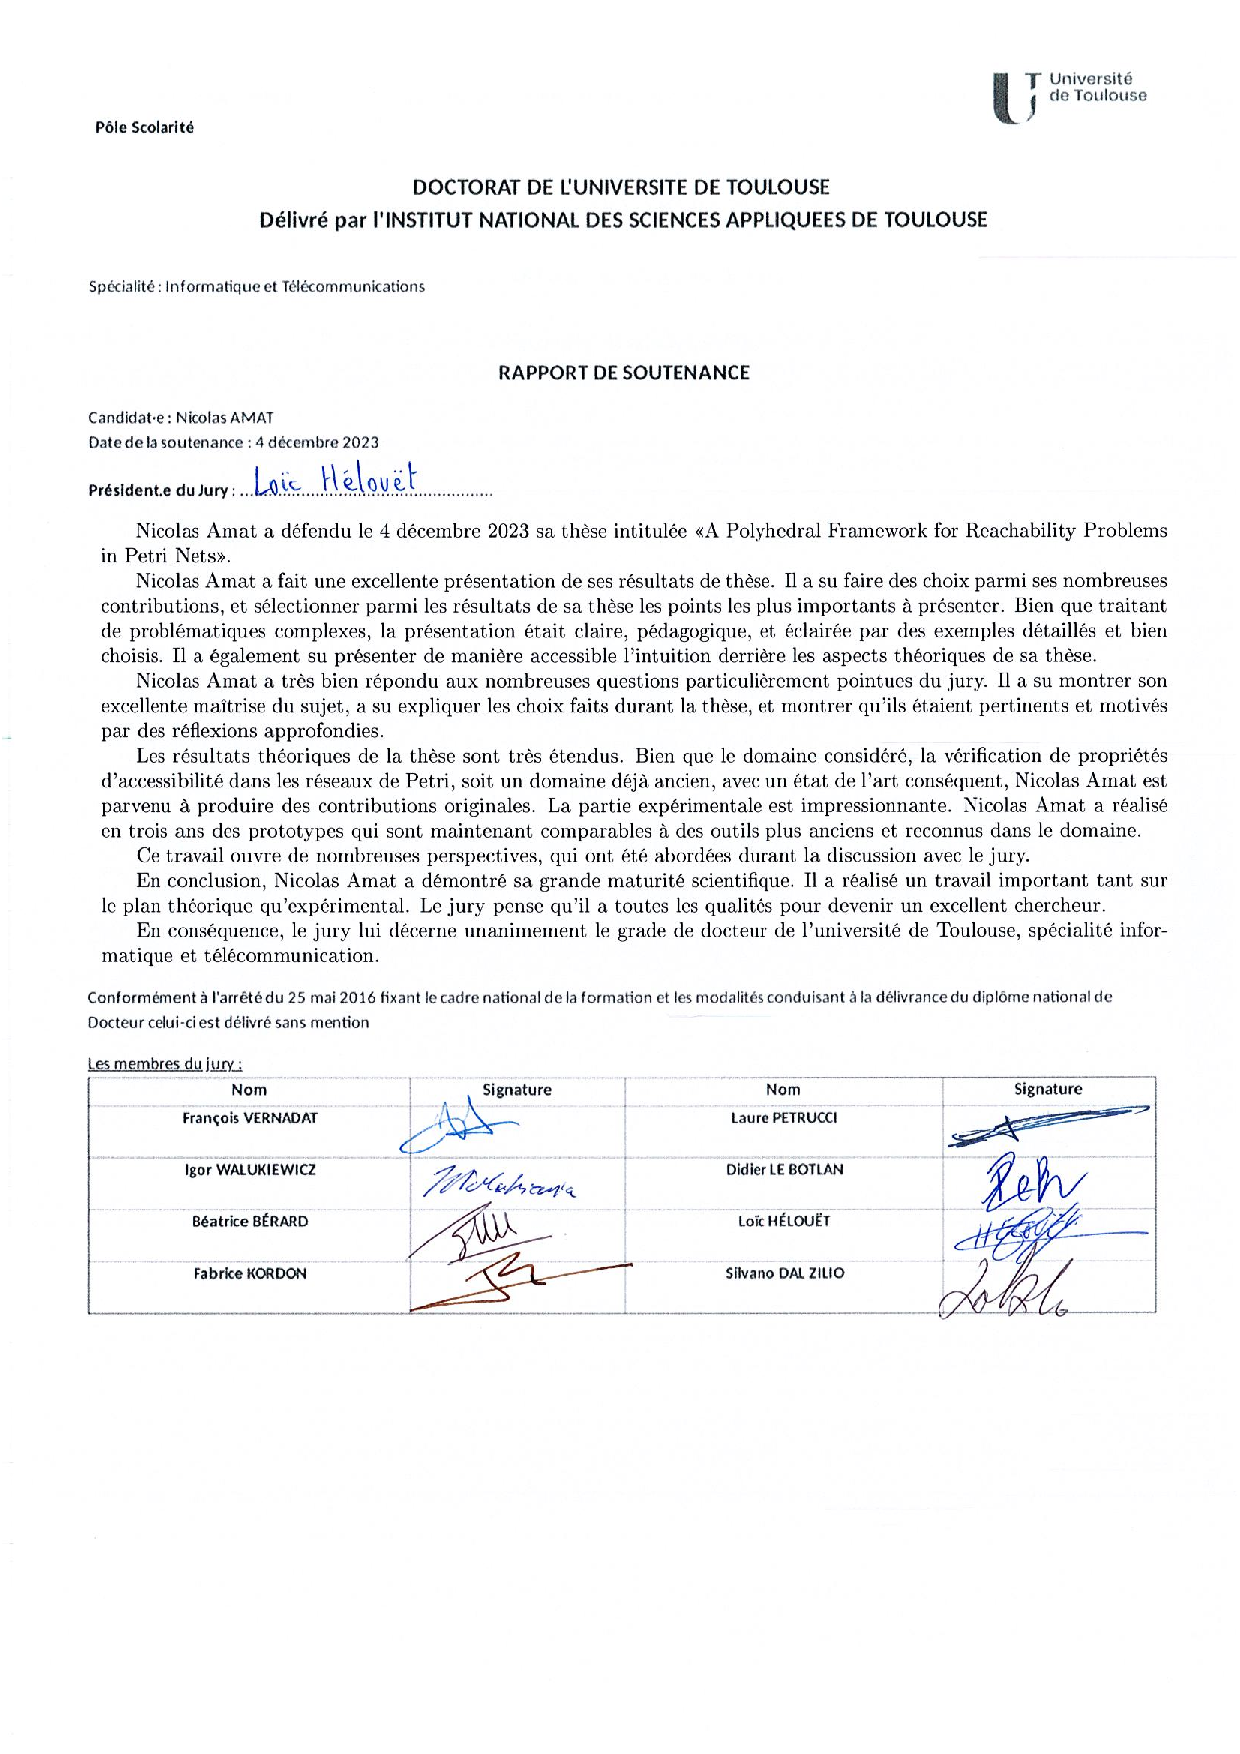
\includepdf[pages=-,link,linkname=soutenance,pagecommand={\refstepcounter{includepdfpage}\label{soutenance.\theincludepdfpage}}]{PDF/Rapport_soutenance.pdf}
\phantomsection\addcontentsline{toc}{chapter}{Rapport de thèse de Mme Laure Petrucci}
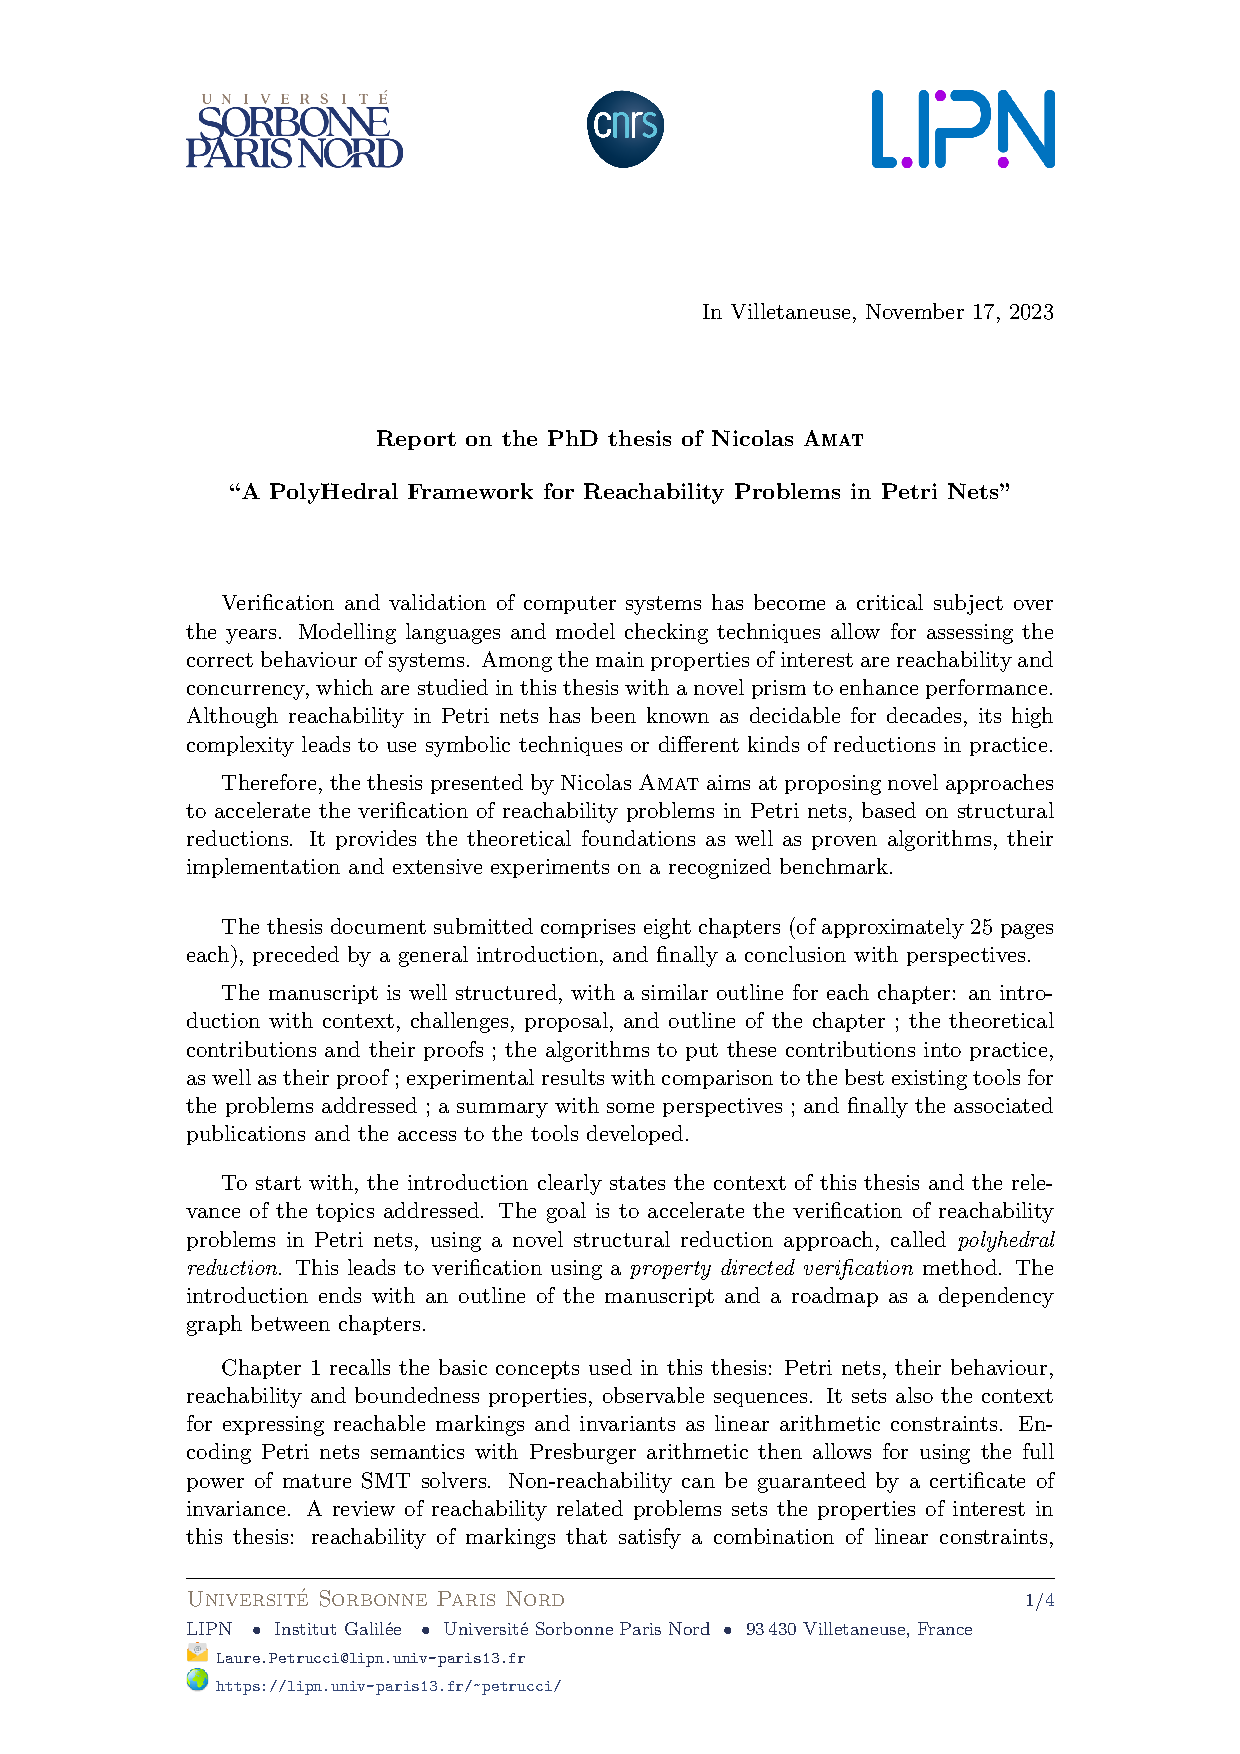
\includepdf[pages=-,link,linkname=petrucci,pagecommand={\refstepcounter{includepdfpage}\label{petrucci.\theincludepdfpage}}]{PDF/Rapport_Laure_Petrucci.pdf}
\phantomsection\addcontentsline{toc}{chapter}{Rapport de thèse de M. Igor Walukiewicz}
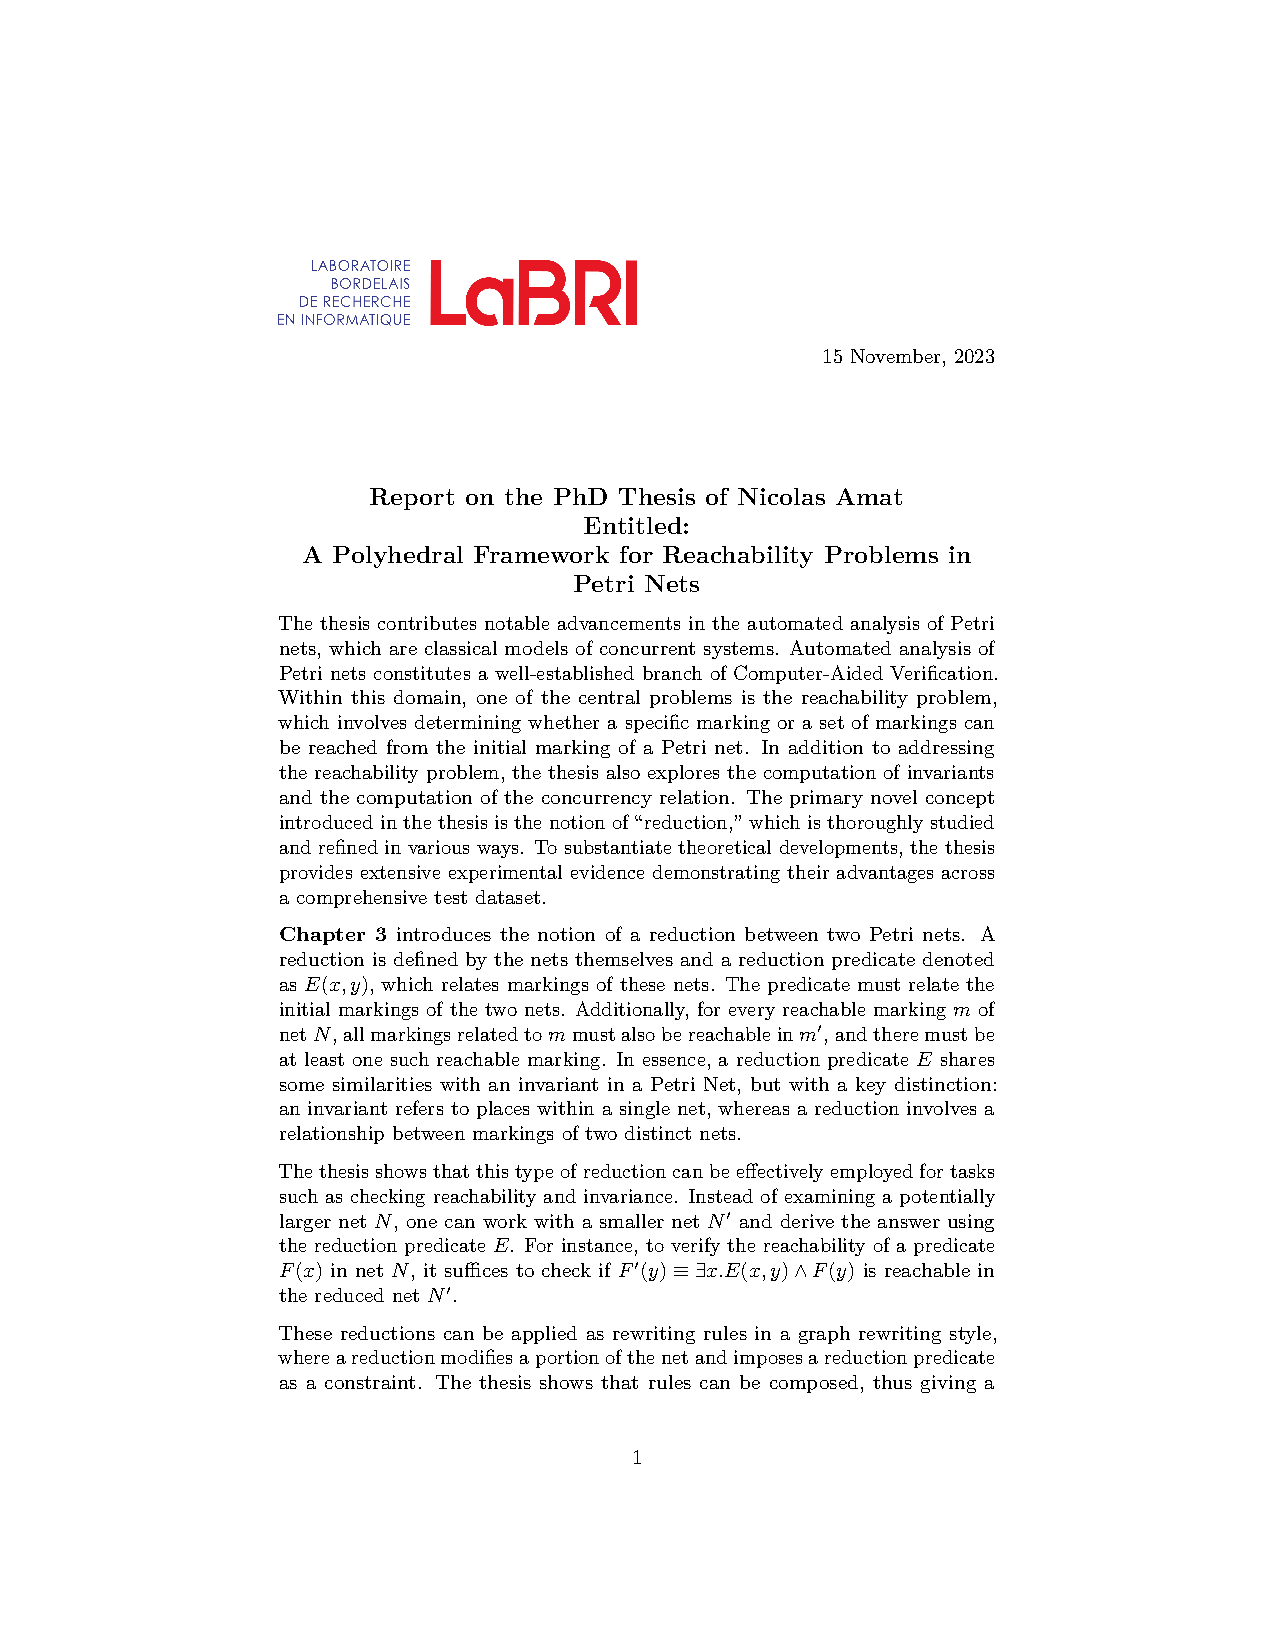
\includepdf[pages=-,link,linkname=walukiewicz,pagecommand={\refstepcounter{includepdfpage}\label{walukiewicz.\theincludepdfpage}}]{PDF/Rapport_Igor_Walukiewicz.pdf}
\phantomsection\addcontentsline{toc}{chapter}{Lettre de soutien (recherche) des encadrants de thèse}

\includepdf[pages=1-2,link,linkname=encadrants,pagecommand={\refstepcounter{includepdfpage}\label{encadrants.\theincludepdfpage}}]{PDF/Lettre_encadrants.pdf}
\phantomsection\addcontentsline{toc}{chapter}{Lettre de soutien (recherche) de M. Fabrice Kordon}

\includepdf[pages=1-2,link,linkname=kordon,pagecommand={\refstepcounter{includepdfpage}\label{kordon.\theincludepdfpage}}]{PDF/Lettre_Fabrice_Kordon.pdf}
\phantomsection\addcontentsline{toc}{chapter}{Lettre de soutien (enseignement) de M. Didier Le Botlan}

\includepdf[pages=1,link,linkname=lebotlan,pagecommand={\refstepcounter{includepdfpage}\label{lebotlan.\theincludepdfpage}}]{PDF/Lettre_Didier_Le_Botlan.pdf}
\phantomsection\addcontentsline{toc}{chapter}{Lettre de soutien (enseignement) de Mme Pauline Ribot}
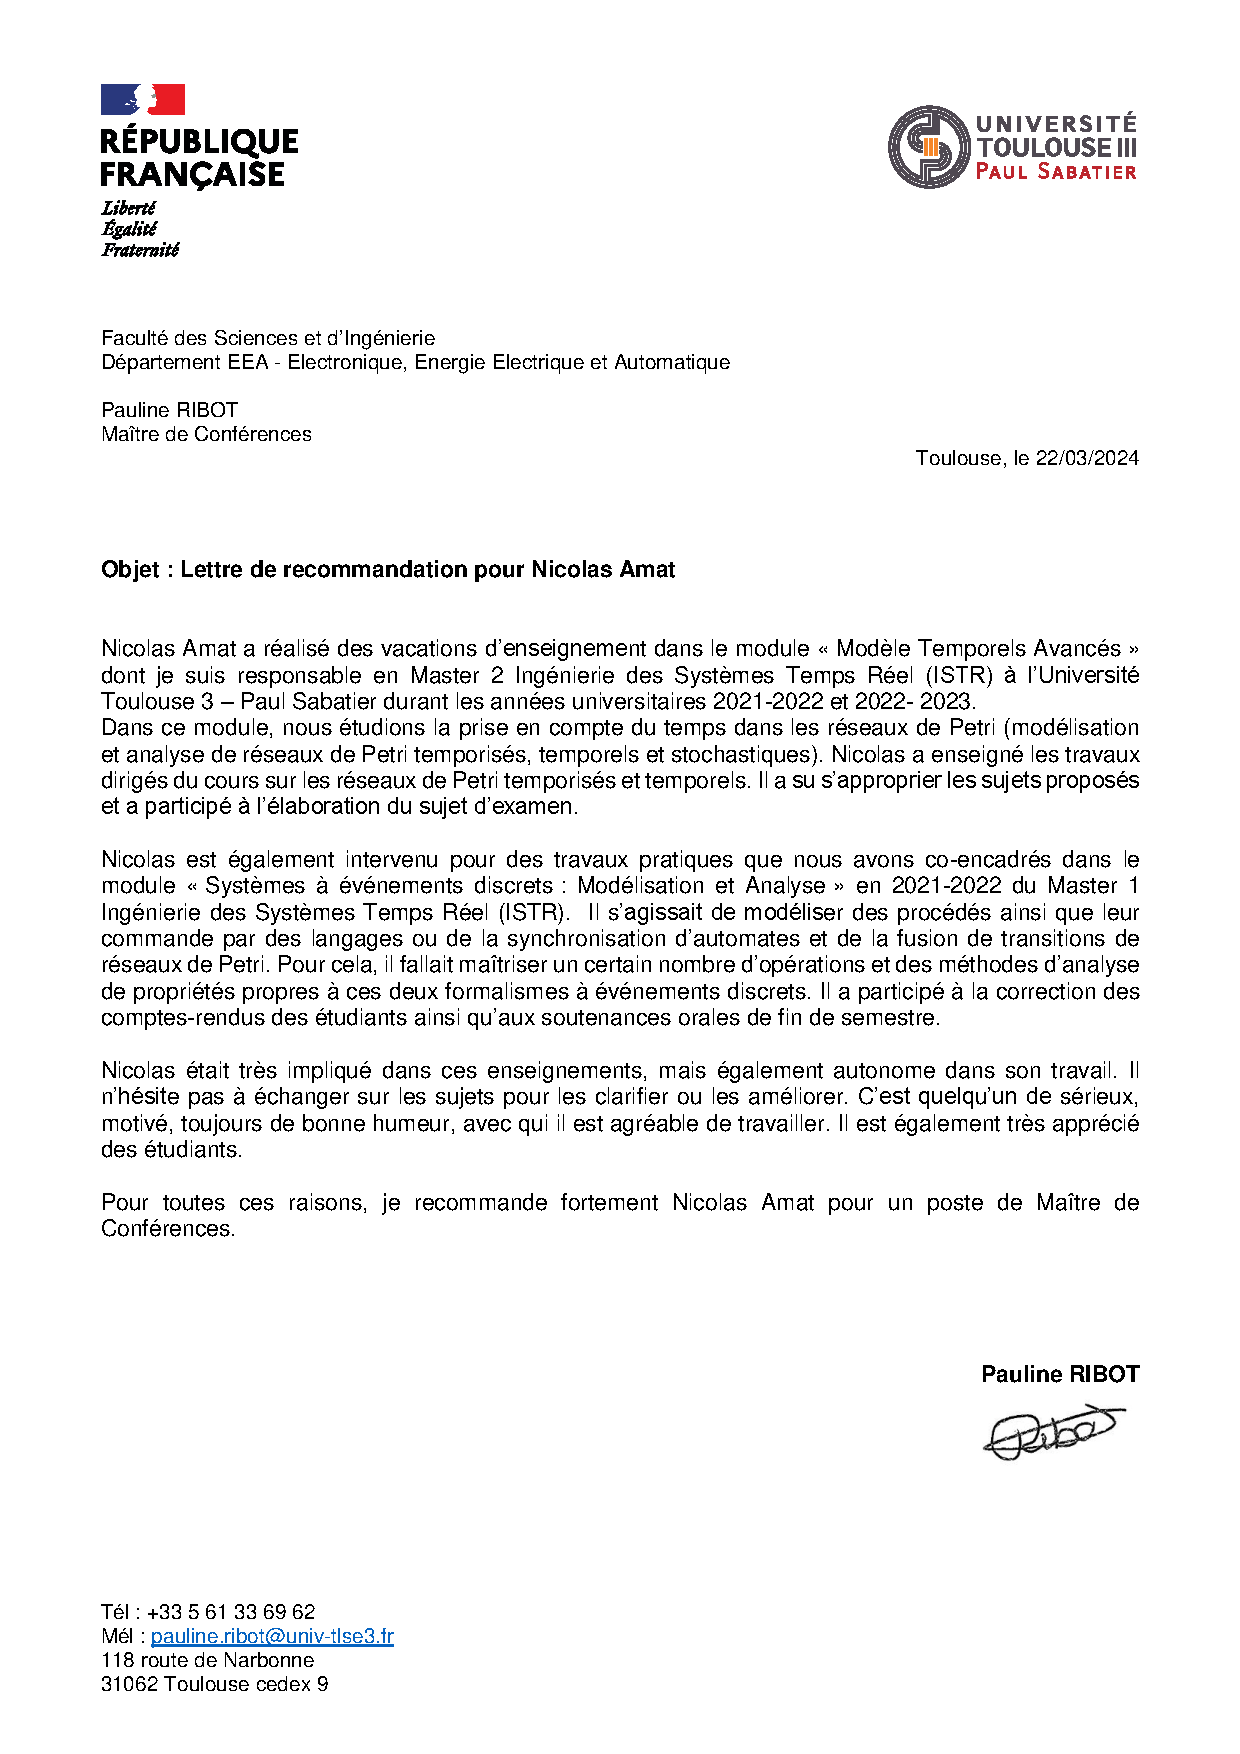
\includepdf[pages=1,link,linkname=ribot,pagecommand={\refstepcounter{includepdfpage}\label{ribot.\theincludepdfpage}}]{PDF/Lettre_Pauline_Ribot.pdf}
\end{document}
